\documentclass[a4paper,parskip,headheight=38pt]{scrartcl} % article or scrartcl
\usepackage[utf8]{inputenc}
\usepackage[T1]{fontenc}
\usepackage{amsmath,amssymb,amsfonts}
\usepackage[%
  automark,
  headsepline                %% Separation line below the header
]{scrlayer-scrpage}
\usepackage[english]{babel}
\usepackage{hyphenat}
\usepackage[hidelinks]{hyperref}
\usepackage[top=1.4in, bottom=1.5in, left=1in, right=1in]{geometry}
\usepackage{lastpage}
\usepackage{csquotes}
\usepackage{microtype}
\usepackage{datetime}

\usepackage[normalem]{ulem}
\usepackage{enumerate}
\usepackage{hyperref}

% \usepackage{multicol}
\usepackage{graphicx}
\usepackage{graphics}
% \usepackage{float}
% \usepackage{caption}

\usepackage{marvosym} % \Lightning

\setkomafont{pagehead}{\normalfont\sffamily\footnotesize}
\addtolength{\headheight}{+6pt}
\lohead{Marlene Böhmer, s9meboeh@stud\ldots, 2547718 \\
	Maximilian Köhl, s8makoeh@stud\ldots, 2553525 \\
	Ben Wiederhake, s9bewied@stud\ldots, 2541266}
\rohead{\newline \newline ES16, Set 5, Page {\thepage}/{\pageref*{LastPage}}}

\newtimeformat{mytime}{\twodigit{\THEHOUR}\twodigit{\THEMINUTE}\twodigit{\THESECOND}}
\settimeformat{mytime}
\newdateformat{mydate}{\twodigit{\THEYEAR}\twodigit{\THEMONTH}\twodigit{\THEDAY}}
\cfoot{\tiny\texttt{ID \mydate\today\currenttime}}
\chead{} % Needed because now the \subsections get displayed
\pagestyle{scrheadings}

% \renewcommand{\headrulewidth}{0pt}
% \addtolength{\textheight}{+30mm}
% \addtolength{\textwidth}{+50mm}
% \addtolength{\hoffset}{-7mm}

% \newcommand{\Omicron}{\ensuremath{\mathcal{O}}}
% \newcommand{\omicron}{\ensuremath{o}}
% \newcommand{\set}[1]{\{#1\}}
% \newcommand{\abs}[1]{\lvert #1 \rvert}

% Thanks to https://tex.stackexchange.com/questions/4216/how-to-typeset-correctly
%\newcommand{\defeq}{\mathrel{\vcenter{\baselineskip0.5ex \lineskiplimit0pt
%                    \hbox{\scriptsize.}\hbox{\scriptsize.}}}%
%                    =}

%\DeclareMathOperator{\sinc}{sinc}

\begin{document}

\section*{Problem 1: Scheduling Algorithms}

\subsection*{Part 1}

I choose to start with EDF and backtrack when necessary (after all,
there's only 3 tasks, so there's only 6 permutations, so backtracking
won't hurt too much).

Until $t=1$, there's no way to do anything.
 \\
At $t=1$, both $J_1, J_2$ become available.  EDF would choose $J_3$
now, so let's go with that.
 \\
At $t=1+C_3=4$, we realize that we missed the deadline for $J_2$.
Dangit.  We must go back!\footnote{In case you don't know:
\url{https://www.google.com/search?q=We\%20must\%20go\%20back!&tbm=isch}}

Back at $t=1$, we choose to do $J_1$ instead, so that $J_2$
can be completed in time.
 \\
At $t=3$, we completed $J_1$ and begin with $J_2$, which is already
available.
 \\
At $t=4$, we completed $J_2$, and don't even start with $J_3$, because
that's not going to work.

\emph{Again} at $t=1$, we choose to do nothing, as obviously both
choices are wrong.
 \\
At $t=2$, we start with $J_2$ as our apparently first activity.
 \\
At $t=3$, we completed $J_2$.  Now EDF would choose $J_3$, so we try
that.
 \\
At $t=6$, we find that we completed $J_2$ just in time, and start with
$J_1$ (just as EDF or any other sane algorithm would).
 \\
At $t=8$, we completed $J_1$, and are done with the task set, meaning
that $(2, J_2), (3, J_3), (6, J_1)$ is a feasible schedule.
 \\
At $t=9$, we sell the time machine and become millionaires.

\subsection*{Part 2}

There exists a feasible EDF schedule for $\Gamma$, as the processor
utilization is $\approx 0.96 \leq 1$.  For RM, we apply the
\enquote{schedulability check} from the lecture:

% Periods are: 3, 4, 8
% C_i are:     1, 2, 1
\[\begin{array}{lll}
R_1^0 = C_1 = 1 & R_2^0 = C_2 = 2 & R_3^0 = C_3 = 1 \\
R_1^1 = 1 \checkmark & R_2^1 = 2 + 1 = 3 & R_3^1 = 1 + 1 + 2 = 4 \\
& R_2^2 = 2 + 1 = 3 \checkmark & R_3^2 = 1 + 2 + 2 = 5 \\
& & R_3^3 = 1 + 2 + 4 = 7 \\
& & R_3^4 = 1 + 3 + 4 = 8 \\
& & R_3^5 = 1 + 3 + 4 = 8 \checkmark \\
\end{array}\]

For $\Delta$, there is no feasible schedule, as the processor
utilization is $\frac{1}{2}+\frac{1}{3}+\frac{1}{4} \gg 1$, and thus
there is no EDF or RM schedule.

For $\Gamma$, there exists a feasible EDF schedule, as the processor
utilization is $1 \leq 1$.  For RM, we again apply the
\enquote{schedulability check} from the lecture:

% Periods are: 2, 5, 8, 20
% C_i are:     1, 1, 2,  1
\[\begin{array}{llll}
R_1^0 = C_1 = 1 & R_2^0 = C_2 = 1 & R_3^0 = C_3 = 2 & R_4^0 = C_4 = 1 \\
R_1^1 = 1\checkmark & R_2^1 = 1 + 1 = 2 & R_3^1 = 2 + 1 + 1 = 4 & R_4^1 = 1 + 1 + 1 + 2 = 5 \\
& R_2^2 = 1 + 1 = 2\checkmark & R_3^2 = 2 + 2 + 1 = 5 & R_4^2 = 1 + 3 + 1 + 2 = 7 \\
& & R_3^3 = 2 + 3 + 1 = 6 & R_4^3 = 1 + 4 + 2 + 2 = 9 \\
& & R_3^4 = 2 + 3 + 2 = 7 & R_4^4 = 1 + 5 + 2 + 4 = 12 \\
& & R_3^5 = 2 + 4 + 2 = 8 & R_4^5 = 1 + 6 + 3 + 4 = 14 \\
& & R_3^6 = 2 + 4 + 2 = 8\checkmark & R_4^6 = 1 + 7 + 3 + 4 = 15 \\
& & & R_4^7 = 1 + 8 + 3 + 4 = 16 \\
& & & R_4^8 = 1 + 8 + 4 + 4 = 17 \\
& & & R_4^9 = 1 + 9 + 4 + 6 = 20 \\
& & & R_4^{10} = 1 + 10 + 4 + 6 = 21 \text{\Lightning}
\end{array}\]


\section*{Problem 2: Priority Ceiling Protocol}

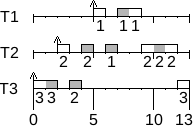
\includegraphics[width=\textwidth]{p3-schedule}

The type of computation is either normal (white box) or critical
section (grey box).
 \\
The numbers are the priorities; changes are indicated as changes.


\section*{Problem 3: Aperiodic Scheduling}

\subsection*{Part a}

FIXME

\subsection*{Part b}

FIXME


\section*{Problem 4: Optimality of Aperiodic scheduling}

\subsection*{Part (a)}

FIXME

\subsection*{Part (b)}

FIXME

\subsection*{Part (c)}

FIXME

\subsection*{Part (d)}

FIXME


\end{document}
